\section{Experiments}\label{experiments}

We evaluate our models on large-scale synthetic and real world data. We compare to neural point process models: \textbf{RMTPP} \cite{RMTPP} and \textbf{Neural hawkes process} \cite{hawkes}. Additionally, we use various RNN models with the knowledge of the time of the next event. We measure the accuracy of class prediction, accuracy of time prediction, and evaluate on an anomaly detection task to show prediction uncertainty.

We split the data into train, validation and test set (60\%--20\%--20\%) and tune all models on a validation set using grid search over learning rate, hidden state dimension and $L_2$ regularization. After running models on all datasets $5$ times we report mean and standard deviation of test set accuracy. Details on model selection can be found in Appendix \ref{model-selection}. The code and further supplementary material is available online.\footnote{\url{https://www.daml.in.tum.de/uncertainty-event-prediction}}

We use the following data (more details in Appendix \ref{datasets}): (1) \textbf{Graph.} We generate data from a directed Erdős–Rényi graph where nodes represent the states and edges the weighted transitions between them. The time it takes to cross one edge is modelled with one normal distribution per edge. By randomly walking along this graph we created $10$K asynchronous events with $10$ unique classes.
(2) \textbf{Stack Exchange.}\footnote{\url{https://archive.org/details/stackexchange}} Sequences contain rewards as events that users get for participation on a question answering website. After preprocessing according to \cite{RMTPP} we have 40 classes and over 480K events spread over 2 years of activity of around 6700 users. The goal is to predict the next reward a user will receive.
(3) \textbf{Smart Home \normalfont\cite{SmartHome}.}\footnote{\url{https://sites.google.com/site/tim0306/datasets}} We use a recorded sequence from a smart house with 14 classes and over $1000$ events. Events correspond to the usage of different appliances. The next event will depend on the time of the day, history of usage and other appliances.
(4) \textbf{Car Indicators.} We obtained a sequence of events from car's indicators that has around $4000$ events with 12 unique classes. The sequence is highly asynchronous, with $\DeltaTime$ ranging from milliseconds to minutes.

\textbf{Visualization.} To analyze the behaviour of the models, we propose visualizations of the evolutions of the parameters predicted by \DirModel and \GPModel.

\textit{Set-up:} We use two toy datasets where the probability of an event depends only on time. The first one (\textbf{3-G}) has three classes occuring at three distinct times. It represents the events in the Fig.\ \ref{fig:car_categorical}. The second one (\textbf{Multi-G}) consists of two classes where one of them has two modes and corresponds to the Fig.\ \ref{fig:kitchen_categorical}. We use these datasets to showcase the importance of time when predicting the next event. In Fig.\ \ref{fig:visualization}, the four top plots show the evolution of the categorical distribution for the \DirModel and the logits for the \GPModel with $10$ points each. The four bottom plots describe the certainty of the models on the probability prediction by plotting the probability $q_\IndexClass(\DeltaTime)$ that the probability of class $\IndexClass$ is higher than others, as introduced in Sec.\ \ref{model_description}.
% These values are computed with sampling methods for \DirModel and with a closed-form expression for \GPModel which explains the difference in the smoothness of these curves.
Additionally, the evolution of the dirichlet distribution over the probability simplex is presented in Appendix \ref{dirichlet_triangle_evolution}.

\begin{figure}
\centering
    \begin{subfigure}{.24\textwidth}
        \centering
        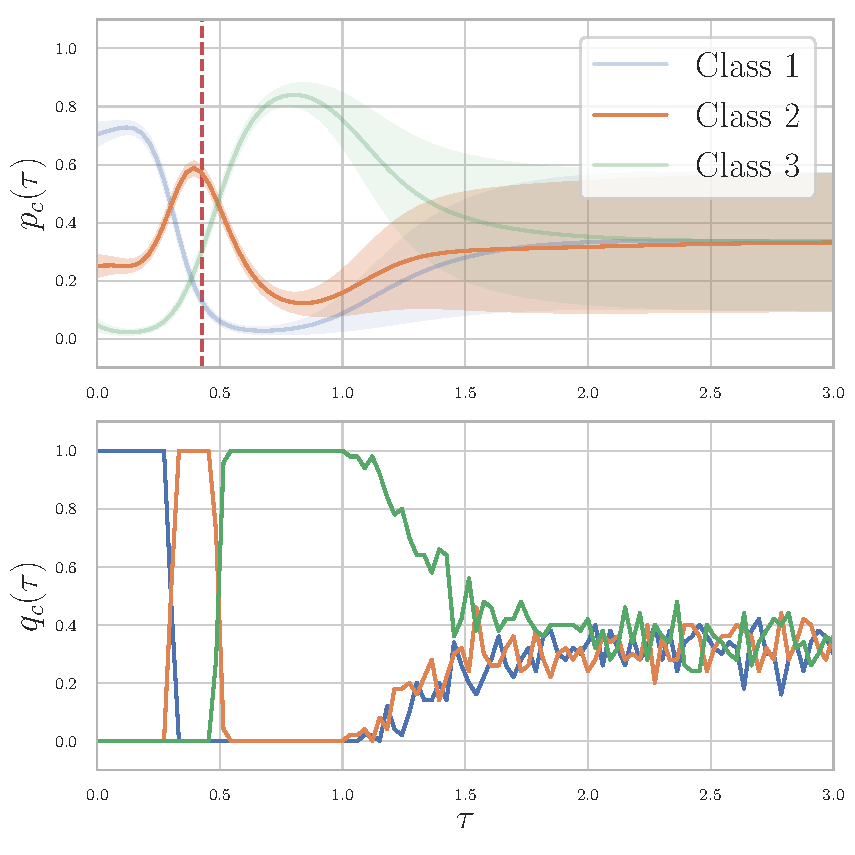
\includegraphics[width=\linewidth]{images/shifted-gaussians-dirichlet.pdf}
        \caption*{\DirModel on 3-G}
    \end{subfigure}
    \begin{subfigure}{.24\textwidth}
        \centering
        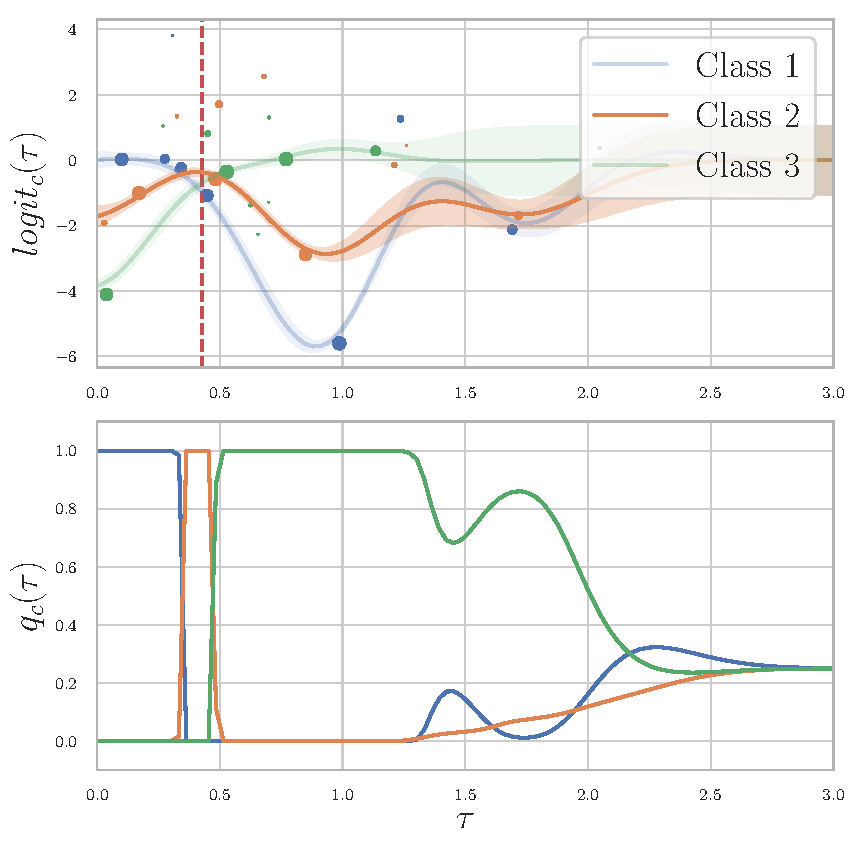
\includegraphics[width=\linewidth]{images/shifted-gaussians-gaussian-process.pdf}
        \caption*{\GPModel on 3-G}
    \end{subfigure}
        \begin{subfigure}{.24\textwidth}
        \centering
        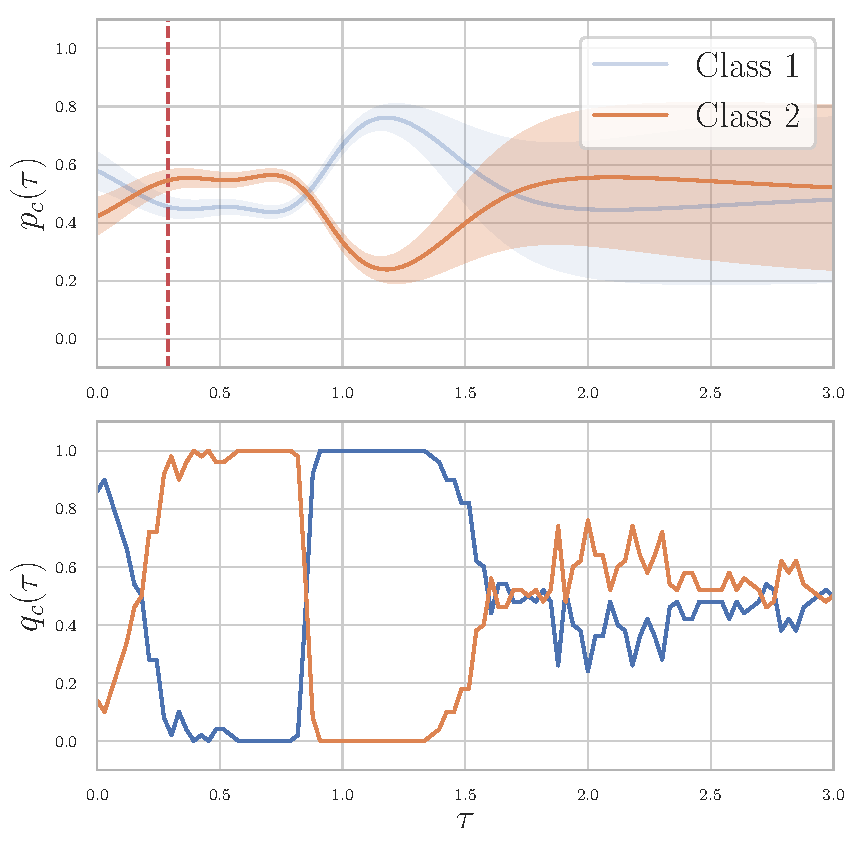
\includegraphics[width=\linewidth]{images/shifted-gaussians-multi-dirichlet.pdf}
        \caption*{\DirModel on Multi-G}
    \end{subfigure}
    \begin{subfigure}{.24\textwidth}
        \centering
        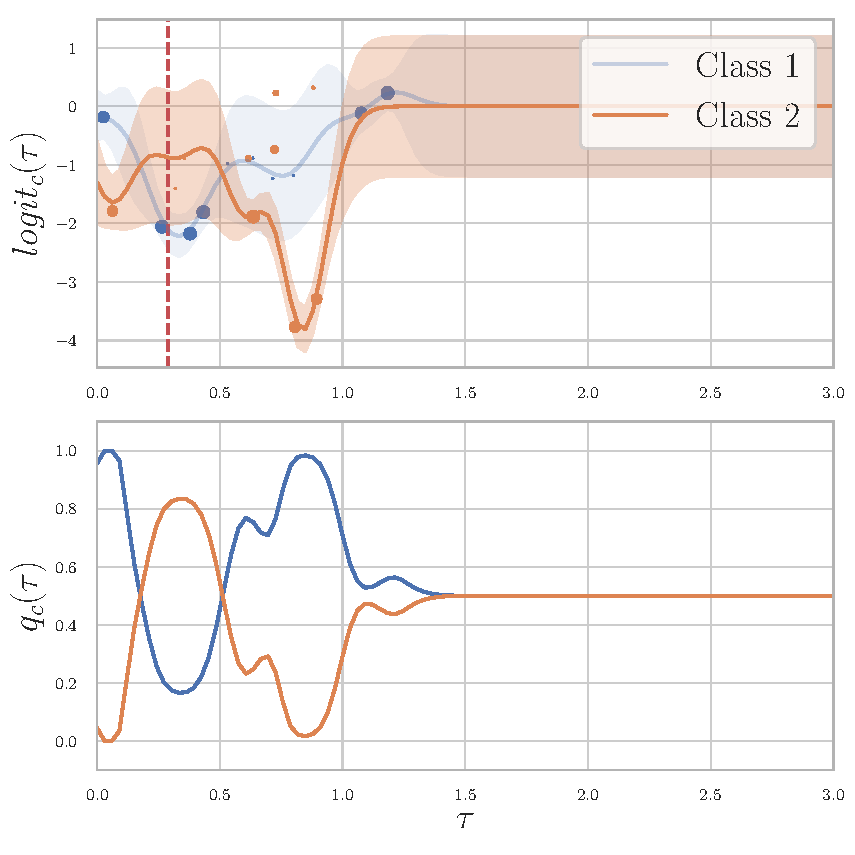
\includegraphics[width=\linewidth]{images/shifted-gaussians-multi-gaussian-process.pdf}
        \caption*{\GPModel on Multi-G}
    \end{subfigure}
    \caption{Visualization of the prediction evolution. The red line indicates the true time of the next event for an example sequence. Here, both models predict the orange class, which is correct, and capture the variation of the class distributions over time. Generated points from \GPModel are plotted with the size corresponding to the weight. For predictions in the far future, both models given high uncertainty.}
    \label{fig:visualization}
    \vspace*{-0.5cm}
\end{figure}

\textit{Results.} Both models learn meaningful evolutions of the distribution on the simplex. For the 3-G data, we can distinguish four areas: the first three correspond to the three classes; after that the prediction is uncertain.
% We remark that the model is certain on the first three areas even if the probability of no class is equal to $1$.
% We can also notice the discarding of points in \GPModel.
The Multi-G data shows that both models are able to approximate multimodal evolutions.
\label{visualization}

\vspace{3mm}
\textbf{Class prediction accuracy.} The aim of this experiment is to assess whether our models can correctly predict the class of the next event, given the time at which it occurs. For this purpose, we compare our models against Hawkes and RMTPP and evalute prediction accuracy on the test set.

\textit{Results.} We can see (Fig. \ref{fig:accuracy}) that our models consistently outperform the other methods on all datasets. Results of the other baselines can be found in Appendix \ref{detail-results}.


\begin{figure}
\centering
    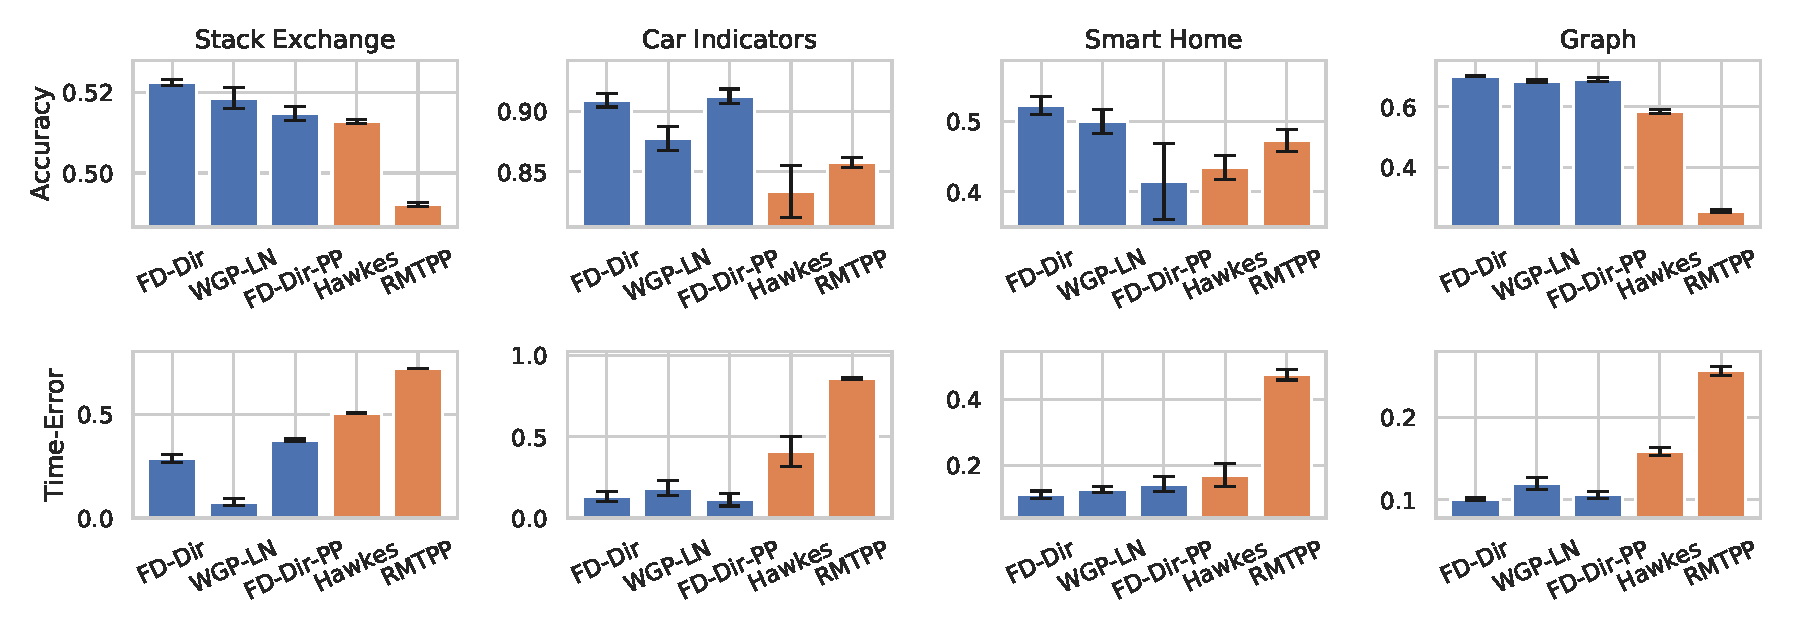
\includegraphics[width=\linewidth]{sections/010_neurips2019/paper/images/accuracy-final.pdf}
    \vspace*{-0.7cm}
    \caption{Class accuracy (top; higher is better) and \TimeScore (bottom; lower is better).}
    \label{fig:accuracy}
    \vspace*{-0.3cm}
\end{figure}
\label{event_prediction}

\textbf{\TimeScore evaluation.} Next, we aim to assess the quality of the time intervals at which we have confidence in one class. Even though \GPModel and the \DirModel do not model a distribution on time, they still have intervals at which we are certain in a class prediction, making the conditional probability a good indicator of the time occurrence of the event.

\textit{Set-up.}  While models predicting a \textit{single} time $\smash{\hat \DeltaTime_i}$ for the next event often use the MSE score $\smash{\frac{1}{n} \sum_{i=1}^n (\hat \DeltaTime_i -\DeltaTime_i^*)^2}$, in our case the MSE is not suitable since one event can occur at multiple time points. In the conventional least-squares approach, the mean of the true distribution is an optimal prediction; however, here it is almost always wrong. Therefore, we use another metric which is better suited for multimodal distributions. Assume that a model returns a score function $\smash{g_\IndexEvent^{(\IndexClass)}(\DeltaTime)}$ for each class regarding the next event $i$, where a large value means the class $\IndexClass$ is likely to occur at time $\DeltaTime$. We define $\smash{\text{\TimeScore} = \frac{1}{n} \sum_{i=1}^n \int \mathbb{1}_{g_\IndexEvent^{(\IndexClass)}(\DeltaTime) \geq g_\IndexEvent^{(\IndexClass)}(\DeltaTime_{\IndexEvent}^*)} d\DeltaTime}$. The
\TimeScore computes the size of the time intervals where the predicted score is larger than the score of the observed time $\DeltaTime_i^*$. Hence, a performant model would achieve a low \TimeScore if its score function $\smash{g_\IndexEvent^{(\IndexClass)}(\DeltaTime)}$ is high at time $\DeltaTime^*$. As the score function in our models, we use the corresponding class probability $\bar{p}_{\IndexEvent \IndexClass}(\DeltaTime)$.

\textit{Results.} We can see that our models clearly obtain the best results on all datasets. The point process version of \DirModel does not improve the performance. Thus, taking also into account the class prediction performance, we recommend to use our other two models. In Appendix \ref{time_mse} we compare FD-Dir-PP with other neural point process models on  time prediction using the MSE score and achieve similar results.
% \begin{figure}
\centering
\begin{subfigure}{0.4 \linewidth}
\centering

\definecolor{dark_cyan}{rgb}{0,0.28,0.28}
\definecolor{pink}{rgb}{1,0.42,0.72}
\definecolor{light_blue}{rgb}{0.42,0.72,1}
\definecolor{brown}{rgb}{0.57,0.29,0}

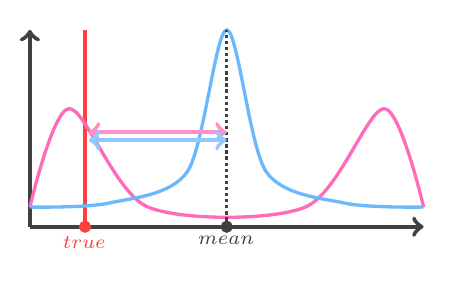
\begin{tikzpicture}[
roundnode/.style={circle, fill=brown!50, very thick, minimum size=11mm},
squarednode/.style={rectangle, fill=dark_cyan!50, very thick, minimum size=10mm},
starnode/.style={regular polygon,regular polygon sides=8, fill=light_blue!66, very thick, minimum size=12mm, inner sep=0},
diamondnode/.style={diamond, fill=pink!66, very thick, minimum size=10mm},]
\draw[black!75, ultra thick, ->] (-5,0.5) -- (0,0.5);
\draw[black!75, ultra thick, ->] (-5,0.5) -- (-5,3);

\draw[red!75, very thick, -] (-4.3,0.5) -- (-4.3,3);
\filldraw[red!75] (-4.3,0.5) circle (2pt) node[anchor=north] {$\DeltaTime^{true}$};

\draw [pink, very thick] plot [smooth, tension=0.5] coordinates { (-5,0.75) (-4.5,2) (-3.5,0.75) (-1.5,0.75) (-0.5,2) (0,0.75)};
\draw [light_blue, very thick] plot [smooth, tension=0.5] coordinates { (-5,0.75) (-4,0.8) (-3,1.2) (-2.5, 3) (-2,1.2) (-1,0.8) (0,0.75)};

\draw[black!75, very thick, densely dotted] (-2.5,0.5) -- (-2.5,3);
\filldraw[black!75] (-2.5,0.5) circle (2pt) node[anchor=north] {$\DeltaTime^{mean}$};

\draw[pink!75, ultra thick, <->] (-4.25,1.7) -- (-2.5,1.7););

\draw[light_blue!75, ultra thick, <->] (-4.25,1.6) -- (-2.5,1.6);

\end{tikzpicture}
\caption{MSE score}\label{fig:MSE_score}
\end{subfigure}
\begin{subfigure}{0.4 \linewidth}
\centering

\definecolor{dark_cyan}{rgb}{0,0.28,0.28}
\definecolor{pink}{rgb}{1,0.42,0.72}
\definecolor{light_blue}{rgb}{0.42,0.72,1}
\definecolor{brown}{rgb}{0.57,0.29,0}

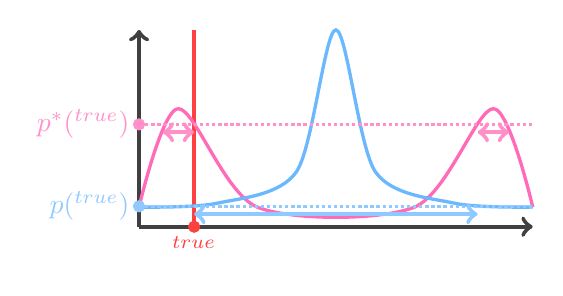
\begin{tikzpicture}[
roundnode/.style={circle, fill=brown!50, very thick, minimum size=11mm},
squarednode/.style={rectangle, fill=dark_cyan!50, very thick, minimum size=10mm},
starnode/.style={regular polygon,regular polygon sides=8, fill=light_blue!66, very thick, minimum size=12mm, inner sep=0},
diamondnode/.style={diamond, fill=pink!66, very thick, minimum size=10mm},]
\draw[black!75, ultra thick, ->] (-5,0.5) -- (0,0.5);
\draw[black!75, ultra thick, ->] (-5,0.5) -- (-5,3);

\draw[red!75, very thick, -] (-4.3,0.5) -- (-4.3,3);
\filldraw[red!75] (-4.3,0.5) circle (2pt) node[anchor=north] {$\DeltaTime^{true}$};

\draw [pink, very thick] plot [smooth, tension=0.5] coordinates { (-5,0.75) (-4.5,2) (-3.5,0.75) (-1.5,0.75) (-0.5,2) (0,0.75)};
\draw [light_blue, very thick] plot [smooth, tension=0.5] coordinates { (-5,0.75) (-4,0.8) (-3,1.2) (-2.5, 3) (-2,1.2) (-1,0.8) (0,0.75)};

\draw[pink!75, very thick, densely dotted] (-5,1.8) -- (0,1.8);
\filldraw[pink!75] (-5,1.8) circle (2pt) node[anchor=east] {$p^*(\DeltaTime^{true})$};
\draw[pink!75, ultra thick, <->] (-4.7,1.7) -- (-4.3,1.7);
\draw[pink!75, ultra thick, <->] (-0.3,1.7) -- (-0.7,1.7);

\draw[light_blue!75, very thick, densely dotted] (-5,0.76) -- (0,0.76);
\filldraw[light_blue!75] (-5,0.76) circle (2pt) node[anchor=east] {$p(\DeltaTime^{true})$};
\draw[light_blue!75, ultra thick, <->] (-4.3,0.66) -- (-0.7,0.66);

\end{tikzpicture}
\caption{\TimeScore}\label{fig:time_score}
\end{subfigure}
\caption{The pink curve is the true time distribution and the blue curve is a uni-modal time distribution.  The value $t^{true}$ is the occurrence time of an event sampled from the true distribution. As it it shows by the arrow the MSE consider that the two distributions have the same quality. In contrast, the \TimeScore estimates that the true distribution is better than the uni-modal distribution}
\end{figure}\label{time_prediction}

\textbf{Anomaly detection \& Uncertainty.} The goal of this experiment is twofold: (1) it assesses the ability of the models to detect anomalies in asynchronous sequences, (2) it evaluates the quality of the predicted uncertainty on the categorical distribution. For this, we use a similar set-up as \citep{PriorNetworks}.

\textit{Set-up:} The experiments consist in introducing anomalies in datasets by changing the occurrence time of $10$\% of the events (at random after the time transformation described in appendix \ref{datasets}). Hence, the anomalies form out-of-distribution data, whereas unchanged events represent in-distribution data. The performance of the anomaly detection is assessed using Area Under Receiver Operating Characteristic (AUROC) and Area Under Precision-Recall (AUPR). We use two approaches: (i) We consider the \textit{categorical uncertainty} on $\bar{\bm{p}}(\DeltaTime)$, i.e., to detect anomalies we use the predicted probability of the true event as the anomaly score. (ii) We use the \textit{distribution uncertainty} at the observed occurrence time provided by our models. For \GPModel, we can evaluate  $q_\IndexClass(\DeltaTime)$ directly (difference of two normal distributions). For \DirModel, this probability does not have a closed-form solution so instead, we use the concentration parameters which are also indicators of out-of-distribution events. For all scores, i.e $\bar{\bm{p}}(\DeltaTime)_c$, $q_\IndexClass(\DeltaTime)$ and $\alpha_\IndexClass(\DeltaTime)$, a low value indicates a potential anomaly around time $\DeltaTime$.

\begin{figure}
\centering
    \begin{subfigure}{0.25\textwidth}
        \centering
        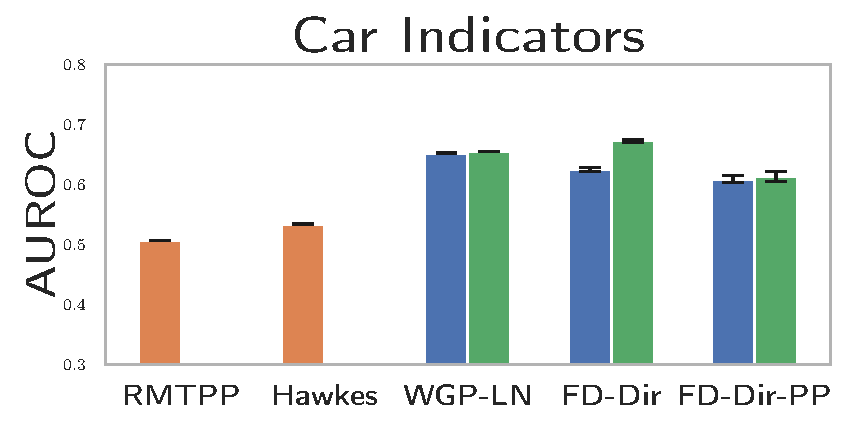
\includegraphics[width=\linewidth]{sections/010_neurips2019/paper/images/uncertainty-roc-bmw-indicator.pdf}
    \end{subfigure}%
    \begin{subfigure}{0.25\textwidth}
        \centering
        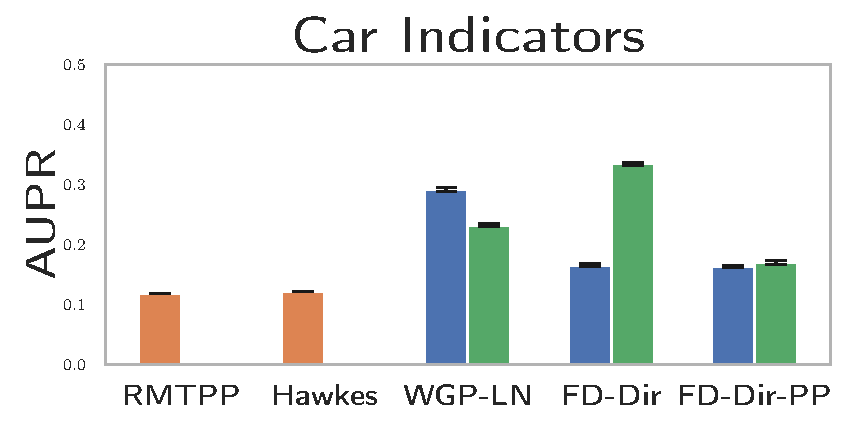
\includegraphics[width=\linewidth]{sections/010_neurips2019/paper/images/uncertainty-apr-bmw-indicator.pdf}
    \end{subfigure}%
        \begin{subfigure}{0.25\textwidth}
        \centering
        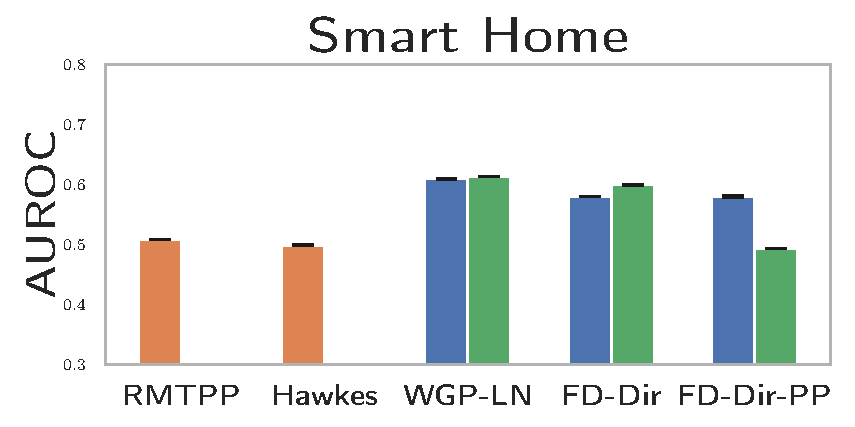
\includegraphics[width=\linewidth]{sections/010_neurips2019/paper/images/uncertainty-roc-kast-home.pdf}
    \end{subfigure}%
    \begin{subfigure}{0.25\textwidth}
        \centering
        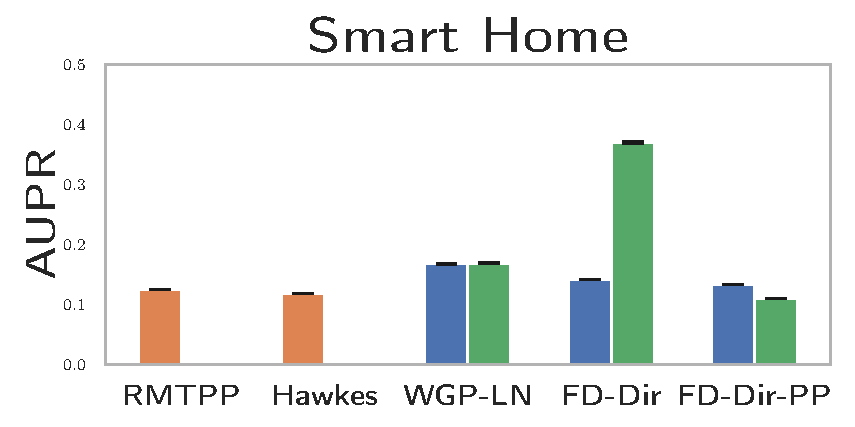
\includegraphics[width=\linewidth]{sections/010_neurips2019/paper/images/uncertainty-apr-kast-home.pdf}
    \end{subfigure}
    \caption{AUROC and APR comparison across dataset on anomaly detection. The orange and blue bars use categorical uncertainty score whereas the green bars use distributional uncertainty.}
    \label{fig:anomaly_detection}
    \vspace{-0.5cm}
\end{figure}

\textit{Results.} As seen in Fig.\ \ref{anomaly_detection}, the \DirModel and the \GPModel have particularly good performance. We observe that the \DirModel gives better results especially with distributional uncertainty. This might be due to the power of the concentration parameters that can be viewed as number of similar events around a given time.\label{anomaly_detection}
